\documentclass{beamer}
\usetheme[numbering = fraction, progressbar = frametitle]{metropolis}           % Use metropolis theme
\usepackage{pgf,tikz,pgfplots}
\pgfplotsset{compat=1.15}
\usepackage{mathrsfs}
\usetikzlibrary{arrows}
\pagestyle{empty}
\usepackage{animate}
\usepackage[font=small,labelfont=bf]{caption}
\usepackage{tikz}
\usetikzlibrary{positioning}


\usepackage[backend=bibtex]{biblatex}
\usepackage{filecontents}
\begin{filecontents}{\jobname.bib}
@article{DBLP:journals/corr/BelloPLNB16,
  author    = {Irwan Bello and
               Hieu Pham and
               Quoc V. Le and
               Mohammad Norouzi and
               Samy Bengio},
  title     = {Neural Combinatorial Optimization with Reinforcement Learning},
  journal   = {CoRR},
  volume    = {abs/1611.09940},
  year      = {2016},
  url       = {http://arxiv.org/abs/1611.09940},
  archivePrefix = {arXiv},
  eprint    = {1611.09940},
  timestamp = {Mon, 13 Aug 2018 16:47:17 +0200},
  biburl    = {https://dblp.org/rec/bib/journals/corr/BelloPLNB16},
  bibsource = {dblp computer science bibliography, https://dblp.org}
}



@article{DBLP:journals/corr/DaiKZDS17,
  author    = {Hanjun Dai and
               Elias B. Khalil and
               Yuyu Zhang and
               Bistra Dilkina and
               Le Song},
  title     = {Learning Combinatorial Optimization Algorithms over Graphs},
  journal   = {CoRR},
  volume    = {abs/1704.01665},
  year      = {2017},
  url       = {http://arxiv.org/abs/1704.01665},
  archivePrefix = {arXiv},
  eprint    = {1704.01665},
  timestamp = {Mon, 13 Aug 2018 16:48:46 +0200},
  biburl    = {https://dblp.org/rec/bib/journals/corr/DaiKZDS17},
  bibsource = {dblp computer science bibliography, https://dblp.org}
}

@article{DBLP:journals/corr/HasseltGS15,
  author    = {Hado van Hasselt and
               Arthur Guez and
               David Silver},
  title     = {Deep Reinforcement Learning with Double Q-learning},
  journal   = {CoRR},
  volume    = {abs/1509.06461},
  year      = {2015},
  url       = {http://arxiv.org/abs/1509.06461},
  archivePrefix = {arXiv},
  eprint    = {1509.06461},
  timestamp = {Mon, 13 Aug 2018 16:47:32 +0200},
  biburl    = {https://dblp.org/rec/bib/journals/corr/HasseltGS15},
  bibsource = {dblp computer science bibliography, https://dblp.org}
}


@article{NIPS2015_5866,
title = {Pointer Networks},
author = {Vinyals, Oriol and Fortunato, Meire and Jaitly, Navdeep},
booktitle = {Advances in Neural Information Processing Systems 28},
editor = {C. Cortes and N. D. Lawrence and D. D. Lee and M. Sugiyama and R. Garnett},
pages = {2692--2700},
year = {2015},
publisher = {Curran Associates, Inc.},
url = {http://papers.nips.cc/paper/5866-pointer-networks.pdf}
}

@article{DBLP:journals/corr/abs-1710-06574,
  author    = {Ruishan Liu and
               James Zou},
  title     = {The Effects of Memory Replay in Reinforcement Learning},
  journal   = {CoRR},
  volume    = {abs/1710.06574},
  year      = {2017},
  url       = {http://arxiv.org/abs/1710.06574},
  archivePrefix = {arXiv},
  eprint    = {1710.06574},
  timestamp = {Mon, 13 Aug 2018 16:46:47 +0200},
  biburl    = {https://dblp.org/rec/bib/journals/corr/abs-1710-06574},
  bibsource = {dblp computer science bibliography, https://dblp.org}
}

@article{DBLP:journals/corr/SchaulQAS15,
  author    = {Tom Schaul and
               John Quan and
               Ioannis Antonoglou and
               David Silver},
  title     = {Prioritized Experience Replay},
  journal   = {CoRR},
  volume    = {abs/1511.05952},
  year      = {2015},
  url       = {http://arxiv.org/abs/1511.05952},
  archivePrefix = {arXiv},
  eprint    = {1511.05952},
  timestamp = {Mon, 13 Aug 2018 16:46:28 +0200},
  biburl    = {https://dblp.org/rec/bib/journals/corr/SchaulQAS15},
  bibsource = {dblp computer science bibliography, https://dblp.org}
}



@article{DBLP:journals/corr/abs-1712-01275,
  author    = {Shangtong Zhang and
               Richard S. Sutton},
  title     = {A Deeper Look at Experience Replay},
  journal   = {CoRR},
  volume    = {abs/1712.01275},
  year      = {2017},
  url       = {http://arxiv.org/abs/1712.01275},
  archivePrefix = {arXiv},
  eprint    = {1712.01275},
  timestamp = {Mon, 13 Aug 2018 16:46:10 +0200},
  biburl    = {https://dblp.org/rec/bib/journals/corr/abs-1712-01275},
  bibsource = {dblp computer science bibliography, https://dblp.org}
}


\end{filecontents}

\addbibresource{\jobname.bib}

\setbeamercolor{normal text}{bg=white}

\usepackage{stmaryrd}

\addtobeamertemplate{navigation symbols}{}{%
    \usebeamerfont{footline}%
    \usebeamercolor[fg]{footline}%
    \hspace{1em}%
    \insertframenumber/\inserttotalframenumber
}

\title{Bandit networks}
\date{January 24, 2019}
\author{Charles \textsc{Auguste} \& Louis \textsc{Trezzini}}
%\institute{Centre for Modern Beamer Themes}
\setbeamercolor{normal text}{bg=white}

\begin{document}

\maketitle

\begin{frame}{Goal of the project}
Study the reinforcement learning framework of 2 articles :
\begin{itemize}
\item \fullcite{DBLP:journals/corr/DaiKZDS17}
\item \fullcite{DBLP:journals/corr/BelloPLNB16}
\end{itemize}
\end{frame}

\begin{frame}{Multi-agent stochastic multi-armed bandit (MAB) problem}
\end{frame}

\begin{frame}{Conclusion}
\begin{itemize}
\item The reinforcement learning methods presented here are \alert{not problem-specific}\end{itemize}
\end{frame}


\begin{frame}{Thank you}
\centering \Huge Any Questions ?
\end{frame}

\begin{frame}
\AtNextBibliography{\tiny}
\printbibliography
\end{frame}

\begin{frame}{Additional slide : Pointer Networks}

\end{frame}


\begin{frame}{Issue with the FYL policy}
\begin{figure}
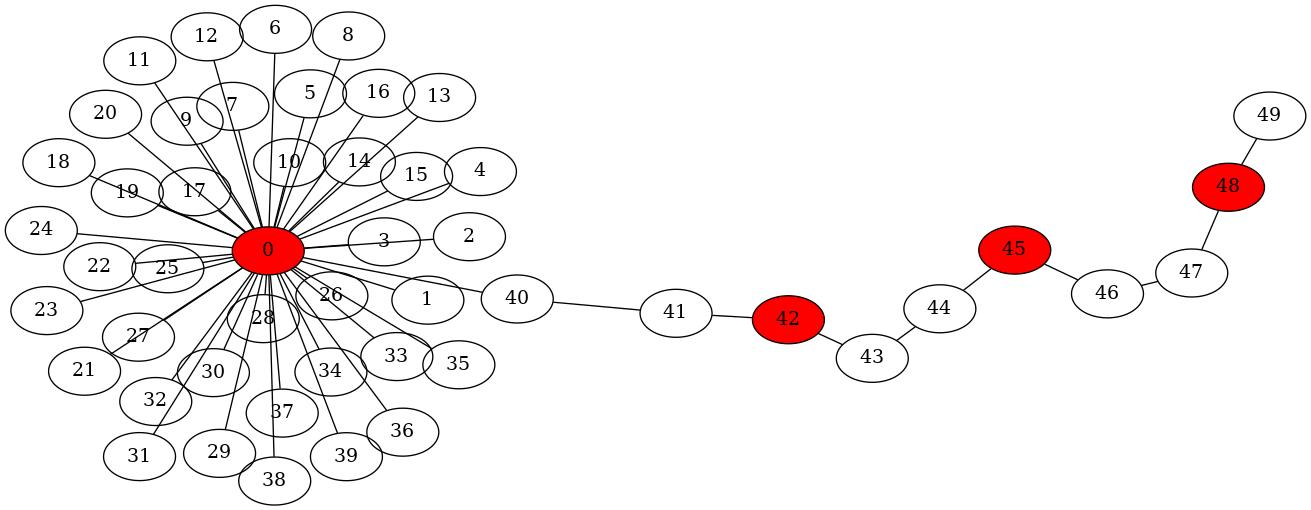
\includegraphics[scale=0.25]{star-chain}
\caption{Star-chain graph, with optimal dominating set in red}
\end{figure}
Nodes 41-49 are \alert{missing on a lot of information} !
\end{frame}

\begin{frame}{Follow Best Informed (FBI) policy}
\begin{itemize}
\item FYL policy is myopic 
\item In addition to their previous action, nodes can output the number of samples (information) they used to compute it
\item Nodes can \alert{follow their best informed neighbor and use UCB-policy if they are better informed}
\item Actually, the structure of a graph fully determines the behavior of the nodes (but not their precise actions obviously)
\end{itemize}
\end{frame}

\begin{frame}{Example of the usefulness of the FBI policy}
\begin{figure}
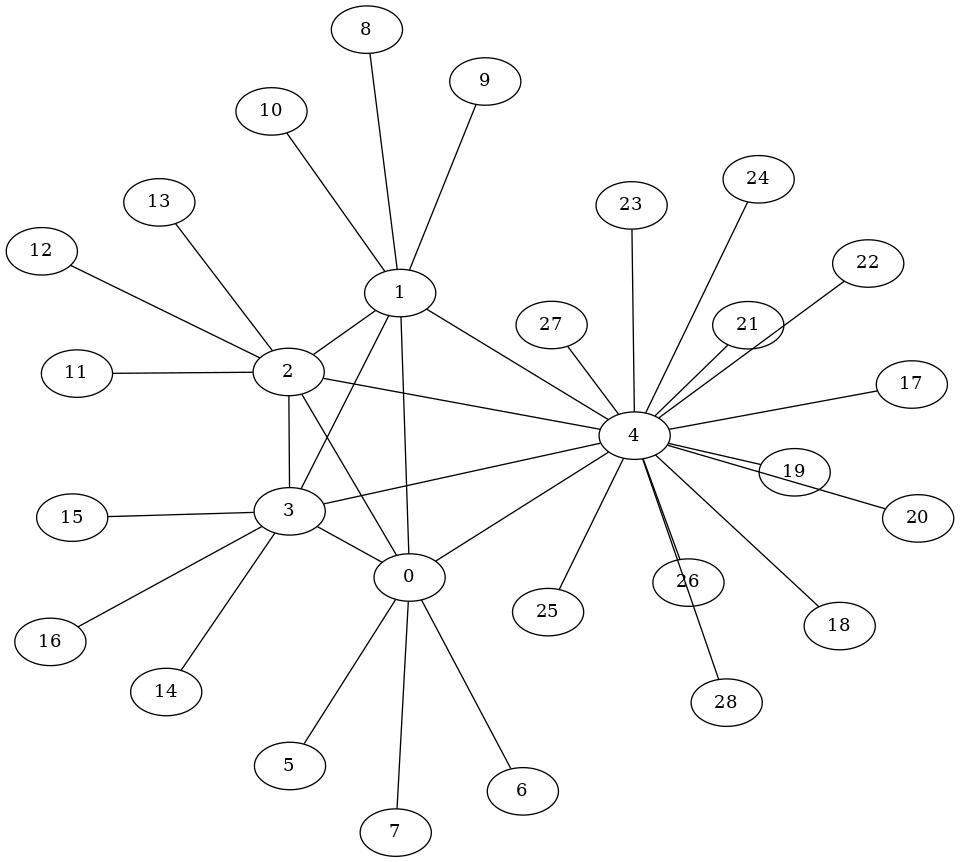
\includegraphics[scale=0.18]{fcstars}
\caption{\centering Fully connected stars graph}
After first iteration, node 4 has the most information. It can pass it to nodes 0-3, who will then pass it to their children. 
\end{figure}
\end{frame}

\begin{frame}{Results for a fully connected stars graph}
\begin{figure}[H]
  \centering
  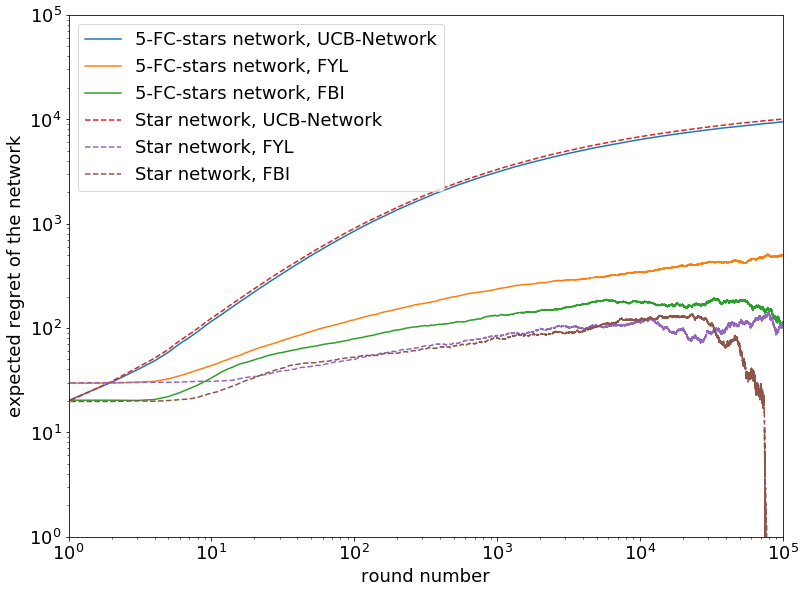
\includegraphics[width=0.49\linewidth]{fig4_1.png}
  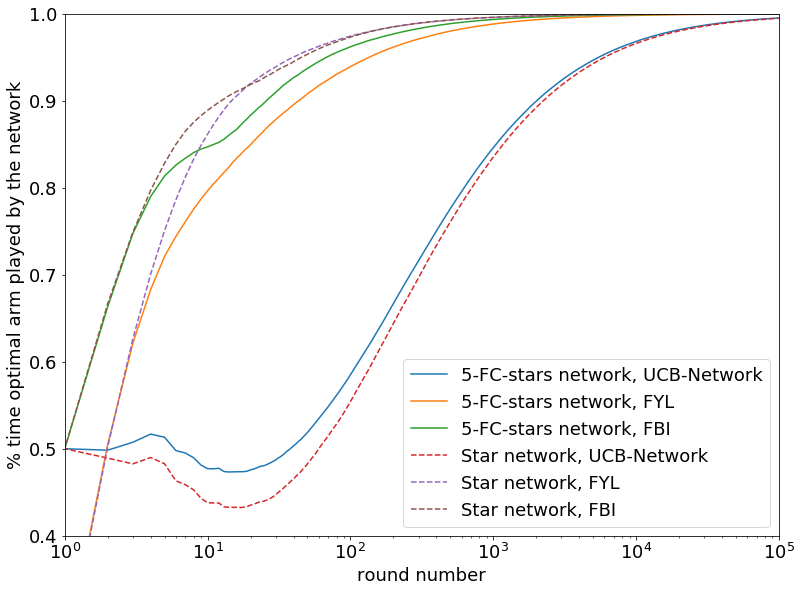
\includegraphics[width=0.49\linewidth]{fig4_2.png}
  \caption{\centering Performance comparison of UCB-Network, FYL, and FBI policies on a 100-nodes star network and on the 100-nodes 5-FC-stars network: 2 arms, Bernoulli rewards with means $0.5$ and $0.7$ (1000 sample paths).}
\end{figure}
\end{frame}

\begin{frame}{Results star-chain graph}
\begin{figure}[H]
  \centering
  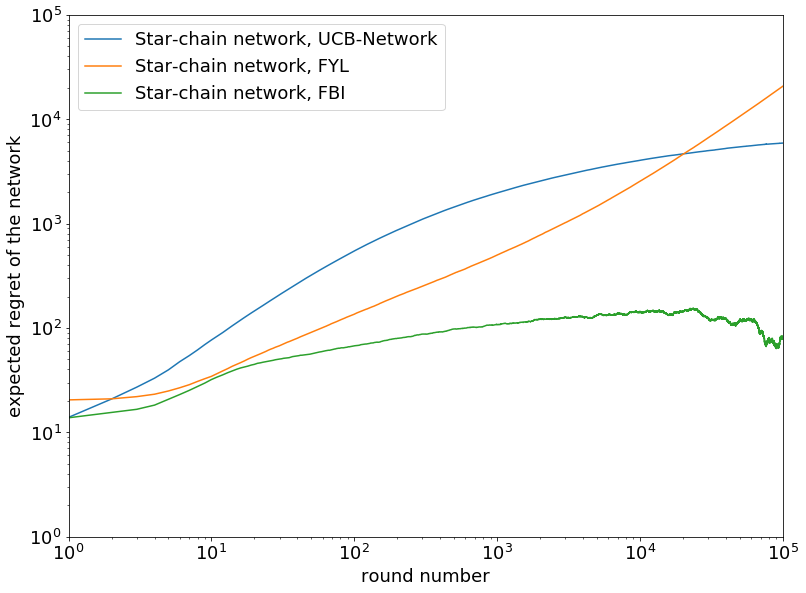
\includegraphics[width=0.49\linewidth]{fig5_1.png}
  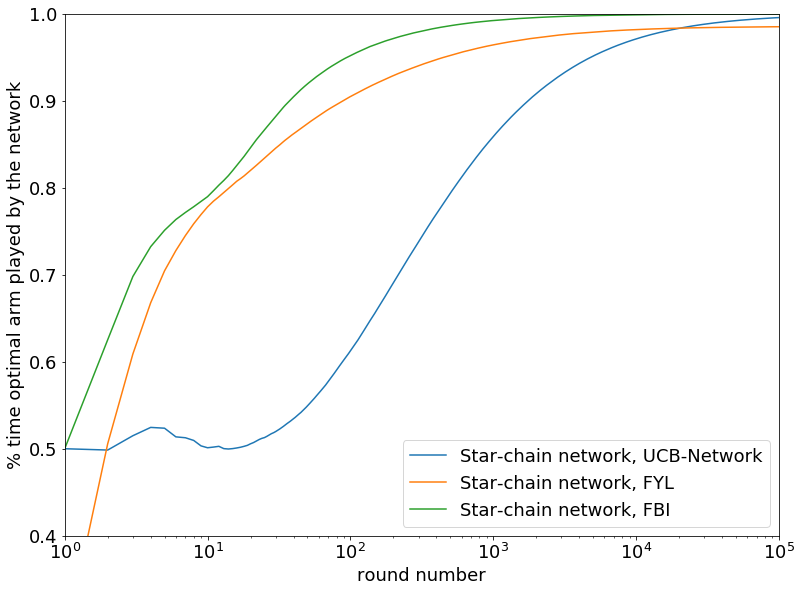
\includegraphics[width=0.49\linewidth]{fig5_2.png}
  \caption{\centering Performance comparison of FYL and FBI policies on the pathological graph structure (star graph with 70 nodes, among which a 20-nodes long chain): 2 arms, Bernoulli rewards with means $0.5$ and $0.7$ (1000 sample paths).}
\end{figure}
\end{frame}

\begin{frame}{A deeper look at the FBI policy}
\begin{itemize}
\item \textbf{Downside} : If one node has more information than the rest, every node it going to follow it (at a delayed rate) $\Rightarrow$ \alert{Strong correlation in the nodes actions} \\ ~ \\


\item \textbf{Further improvements} : When a node has multiple neighbors informed about in the same way, it may be smart to randomly follow one with a \alert{probability depending on its amount of information}. But then the behavior of the nodes is not determined by the structure of the graph... 
\end{itemize}
\end{frame}




\end{document}
